\documentclass[11pt,a4paper,]{article}
\usepackage{lmodern}

\usepackage{amssymb,amsmath}
\usepackage{ifxetex,ifluatex}
\usepackage{fixltx2e} % provides \textsubscript
\ifnum 0\ifxetex 1\fi\ifluatex 1\fi=0 % if pdftex
  \usepackage[T1]{fontenc}
  \usepackage[utf8]{inputenc}
\else % if luatex or xelatex
  \usepackage{unicode-math}
  \defaultfontfeatures{Ligatures=TeX,Scale=MatchLowercase}
\fi
% use upquote if available, for straight quotes in verbatim environments
\IfFileExists{upquote.sty}{\usepackage{upquote}}{}
% use microtype if available
\IfFileExists{microtype.sty}{%
\usepackage[]{microtype}
\UseMicrotypeSet[protrusion]{basicmath} % disable protrusion for tt fonts
}{}
\PassOptionsToPackage{hyphens}{url} % url is loaded by hyperref
\usepackage[unicode=true]{hyperref}
\hypersetup{
            pdftitle={Attention Towards Distance Education Tools During COVID-19 Pandemic: Evidence from Google Trends},
            pdfkeywords={rmarkdown, templates},
            pdfborder={0 0 0},
            breaklinks=true}
\urlstyle{same}  % don't use monospace font for urls
\usepackage{geometry}
\geometry{left=2.5cm,right=2.5cm,top=2.5cm,bottom=2.5cm}
\usepackage[style=authoryear-comp,]{biblatex}
\addbibresource{references.bib}
\usepackage{longtable,booktabs}
% Fix footnotes in tables (requires footnote package)
\IfFileExists{footnote.sty}{\usepackage{footnote}\makesavenoteenv{long table}}{}
\IfFileExists{parskip.sty}{%
\usepackage{parskip}
}{% else
\setlength{\parindent}{0pt}
\setlength{\parskip}{6pt plus 2pt minus 1pt}
}
\setlength{\emergencystretch}{3em}  % prevent overfull lines
\providecommand{\tightlist}{%
  \setlength{\itemsep}{0pt}\setlength{\parskip}{0pt}}
\setcounter{secnumdepth}{5}

% set default figure placement to htbp
\makeatletter
\def\fps@figure{htbp}
\makeatother


\title{Attention Towards Distance Education Tools During COVID-19 Pandemic: Evidence from Google Trends}

%% MONASH STUFF

%% CAPTIONS
\RequirePackage{caption}
\DeclareCaptionStyle{italic}[justification=centering]
 {labelfont={bf},textfont={it},labelsep=colon}
\captionsetup[figure]{style=italic,format=hang,singlelinecheck=true}
\captionsetup[table]{style=italic,format=hang,singlelinecheck=true}

%% FONT
\RequirePackage{bera}
\RequirePackage{mathpazo}

%% HEADERS AND FOOTERS
\RequirePackage{fancyhdr}
\pagestyle{fancy}
\rfoot{\Large\sffamily\raisebox{-0.1cm}{\textbf{\thepage}}}
\makeatletter
\lhead{\textsf{\expandafter{\@title}}}
\makeatother
\rhead{}
\cfoot{}
\setlength{\headheight}{15pt}
\renewcommand{\headrulewidth}{0.4pt}
\renewcommand{\footrulewidth}{0.4pt}
\fancypagestyle{plain}{%
\fancyhf{} % clear all header and footer fields
\fancyfoot[C]{\sffamily\thepage} % except the center
\renewcommand{\headrulewidth}{0pt}
\renewcommand{\footrulewidth}{0pt}}

%% MATHS
\RequirePackage{bm,amsmath}
\allowdisplaybreaks

%% GRAPHICS
\RequirePackage{graphicx}
\setcounter{topnumber}{2}
\setcounter{bottomnumber}{2}
\setcounter{totalnumber}{4}
\renewcommand{\topfraction}{0.85}
\renewcommand{\bottomfraction}{0.85}
\renewcommand{\textfraction}{0.15}
\renewcommand{\floatpagefraction}{0.8}

%\RequirePackage[section]{placeins}

%% SECTION TITLES
\RequirePackage[compact,sf,bf]{titlesec}
\titleformat{\section}[block]
  {\fontsize{15}{17}\bfseries\sffamily}
  {\thesection}
  {0.4em}{}
\titleformat{\subsection}[block]
  {\fontsize{12}{14}\bfseries\sffamily}
  {\thesubsection}
  {0.4em}{}
\titlespacing{\section}{0pt}{*5}{*1}
\titlespacing{\subsection}{0pt}{*2}{*0.2}


%% TITLE PAGE
\def\Date{\number\day}
\def\Month{\ifcase\month\or
 January\or February\or March\or April\or May\or June\or
 July\or August\or September\or October\or November\or December\fi}
\def\Year{\number\year}

\makeatletter
\def\wp#1{\gdef\@wp{#1}}\def\@wp{??/??}
\def\jel#1{\gdef\@jel{#1}}\def\@jel{??}
\def\showjel{{\large\textsf{\textbf{JEL classification:}}~\@jel}}
\def\nojel{\def\showjel{}}
\def\addresses#1{\gdef\@addresses{#1}}\def\@addresses{??}
\def\cover{{\sffamily\setcounter{page}{0}
        \thispagestyle{empty}
        \vspace*{2cm}
        \begin{center}
        \fbox{\parbox{14cm}{\begin{onehalfspace}\centering\Huge\vspace*{0.3cm}
                \textsf{\textbf{\expandafter{\@title}}}\vspace{1cm}\par
                \LARGE\@author\end{onehalfspace}
        }}
        \end{center}
        \vfill
                \begin{center}\Large
                \Month~\Year\\[1cm]
                Working Paper \@wp
        \end{center}\vspace*{2cm}}}
\def\pageone{{\sffamily\setstretch{1}%
        \thispagestyle{empty}%
        \vbox to \textheight{%
        \raggedright\baselineskip=1.2cm
     {\fontsize{24.88}{30}\sffamily\textbf{\expandafter{\@title}}}
        \vspace{2cm}\par
        \hspace{1cm}\parbox{14cm}{\sffamily\large\@addresses}\vspace{1cm}\vfill
        \hspace{1cm}{\large\Date~\Month~\Year}\\[1cm]
        \hspace{1cm}\showjel\vss}}}
\def\blindtitle{{\sffamily
     \thispagestyle{plain}\raggedright\baselineskip=1.2cm
     {\fontsize{24.88}{30}\sffamily\textbf{\expandafter{\@title}}}\vspace{1cm}\par
        }}
\def\titlepage{{\cover\newpage\pageone\newpage\blindtitle}}

\def\blind{\def\titlepage{{\blindtitle}}\let\maketitle\blindtitle}
\def\titlepageonly{\def\titlepage{{\pageone\end{document}}}}
\def\nocover{\def\titlepage{{\pageone\newpage\blindtitle}}\let\maketitle\titlepage}
\let\maketitle\titlepage
\makeatother

%% SPACING
\RequirePackage{setspace}
\spacing{1.5}

%% LINE AND PAGE BREAKING
\sloppy
\clubpenalty = 10000
\widowpenalty = 10000
\brokenpenalty = 10000
\RequirePackage{microtype}

%% PARAGRAPH BREAKS
\setlength{\parskip}{1.4ex}
\setlength{\parindent}{0em}

%% HYPERLINKS
\RequirePackage{xcolor} % Needed for links
\definecolor{darkblue}{rgb}{0,0,.6}
\RequirePackage{url}

\makeatletter
\@ifpackageloaded{hyperref}{}{\RequirePackage{hyperref}}
\makeatother
\hypersetup{
     citecolor=0 0 0,
     breaklinks=true,
     bookmarksopen=true,
     bookmarksnumbered=true,
     linkcolor=darkblue,
     urlcolor=blue,
     citecolor=darkblue,
     colorlinks=true}

%% KEYWORDS
\newenvironment{keywords}{\par\vspace{0.5cm}\noindent{\sffamily\textbf{Keywords:}}}{\vspace{0.25cm}\par\hrule\vspace{0.5cm}\par}

%% ABSTRACT
\renewenvironment{abstract}{\begin{minipage}{\textwidth}\parskip=1.4ex\noindent
\hrule\vspace{0.1cm}\par{\sffamily\textbf{\abstractname}}\newline}
  {\end{minipage}}


\usepackage[T1]{fontenc}
\usepackage[utf8]{inputenc}

\usepackage[showonlyrefs]{mathtools}
\usepackage[no-weekday]{eukdate}

%% BIBLIOGRAPHY

\makeatletter
\@ifpackageloaded{biblatex}{}{\usepackage[style=authoryear-comp, backend=biber, natbib=true]{biblatex}}
\makeatother
\ExecuteBibliographyOptions{bibencoding=utf8,minnames=1,maxnames=3, maxbibnames=99,dashed=false,terseinits=true,giveninits=true,uniquename=false,uniquelist=false,doi=false, isbn=false,url=true,sortcites=false}

\DeclareFieldFormat{url}{\texttt{\url{#1}}}
\DeclareFieldFormat[article]{pages}{#1}
\DeclareFieldFormat[inproceedings]{pages}{\lowercase{pp.}#1}
\DeclareFieldFormat[incollection]{pages}{\lowercase{pp.}#1}
\DeclareFieldFormat[article]{volume}{\mkbibbold{#1}}
\DeclareFieldFormat[article]{number}{\mkbibparens{#1}}
\DeclareFieldFormat[article]{title}{\MakeCapital{#1}}
\DeclareFieldFormat[inproceedings]{title}{#1}
\DeclareFieldFormat{shorthandwidth}{#1}
% No dot before number of articles
\usepackage{xpatch}
\xpatchbibmacro{volume+number+eid}{\setunit*{\adddot}}{}{}{}
% Remove In: for an article.
\renewbibmacro{in:}{%
  \ifentrytype{article}{}{%
  \printtext{\bibstring{in}\intitlepunct}}}

\makeatletter
\DeclareDelimFormat[cbx@textcite]{nameyeardelim}{\addspace}
\makeatother
\renewcommand*{\finalnamedelim}{%
  %\ifnumgreater{\value{liststop}}{2}{\finalandcomma}{}% there really should be no funny Oxford comma business here
  \addspace\&\space}


\wp{1}
\jel{C10,C14,C22}

\RequirePackage[absolute,overlay]{textpos}
\setlength{\TPHorizModule}{1cm}
\setlength{\TPVertModule}{1cm}
\def\placefig#1#2#3#4{\begin{textblock}{.1}(#1,#2)\rlap{\includegraphics[#3]{#4}}\end{textblock}}




\author{Priyanga Dilini~Talagala, Thiyanga S.~Talagala}
\addresses{\textbf{Priyanga Dilini Talagala}\newline
Department of Compuational Mathematics, University of Moratuwa, Sri Lanka
\newline{Email: \href{mailto:priyangad@uom.lk}{\nolinkurl{priyangad@uom.lk}}}\newline Corresponding author\\[1cm]
\textbf{Thiyanga S. Talagala}\newline
Department of Statistics, University of Sri Jayewardenepura, Sri Lanka
\newline{Email: \href{mailto:tstalagala@gmail.com}{\nolinkurl{tstalagala@gmail.com}}}\\[1cm]
}

\date{\sf\Date~\Month~\Year}
\makeatletter
 \lfoot{\sf Talagala, Talagala: \@date}
\makeatother

%% Any special functions or other packages can be loaded here.


\begin{document}
\maketitle
\begin{abstract}
A brief summary of our work
\end{abstract}
\begin{keywords}
rmarkdown, templates
\end{keywords}

\hypertarget{introduction}{%
\section{Introduction}\label{introduction}}

The ongoing pandemic of COVID-19 is still one of the most important priorities of governments and media of many countries all around the world. Due to the alarming levels of spread and severity, the World Health Organization (WHO) declared the outbreak a Public Health Emergency of International Concern (PHEIC) on 30 January 2020, and then a pandemic on 11 March 2020 \autocite{world2020timeline}. As of 29 September 2021, more than 232.7 million cases of COVID-19 have been reported in over 192 countries and territories, resulting in more than 4.7 million deaths \autocite{dong2020interactive}. In response to the pandemic, health authorities worldwide have taken many steps including vaccination development and deployment to minimize the spread of the virus. In addition, authorities worldwide have also taken many non-pharmaceutical interventions and preventive measures such as travel restrictions, lock-downs, workplace hazard controls, school/university closures, facility closures, reduction of mass gatherings to reduce the spread of the virus \autocite{chang2020modelling}.

\begin{figure}[h]

{\centering 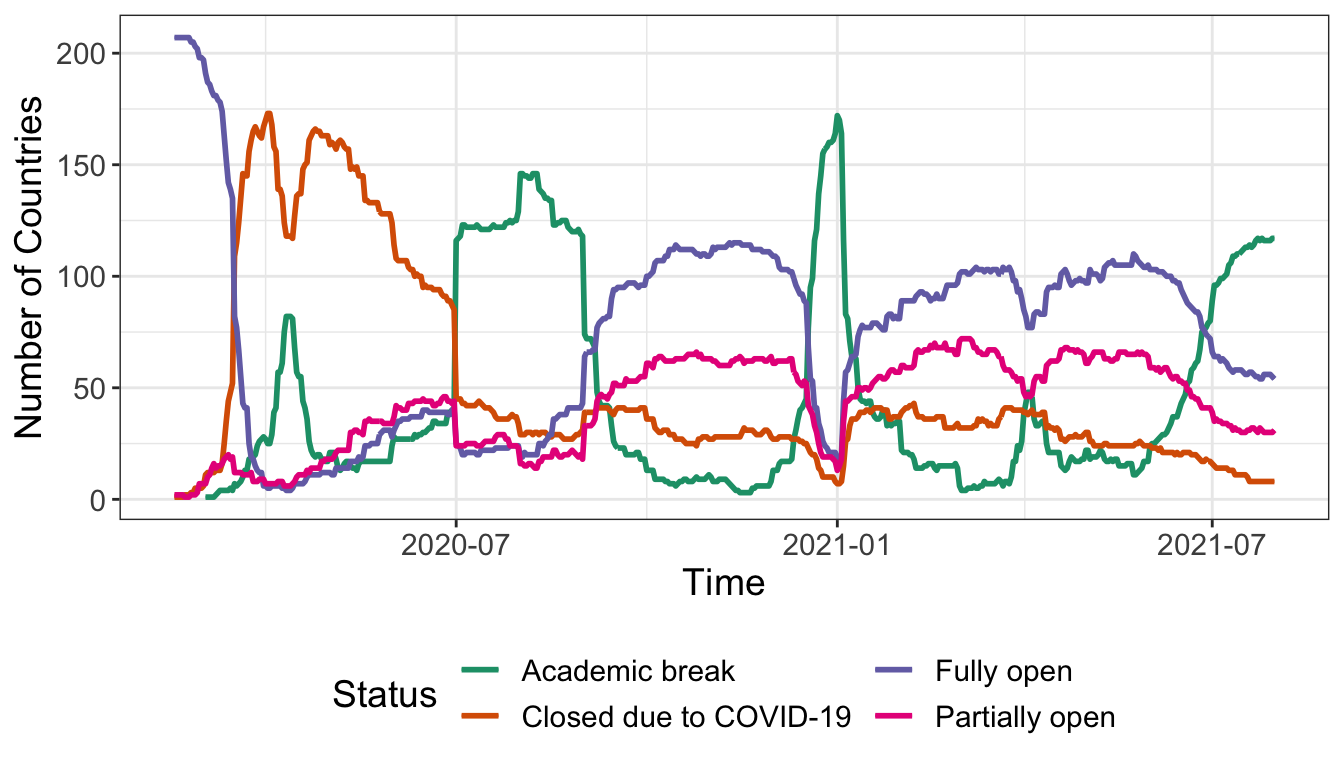
\includegraphics[width=1\textwidth]{figure/covidImpactWorld-1} 

}

\caption{Global tracking of COVID-19 caused school closures and re-openings}\label{fig:covidImpactWorld}
\end{figure}

\begin{figure}[h]

{\centering 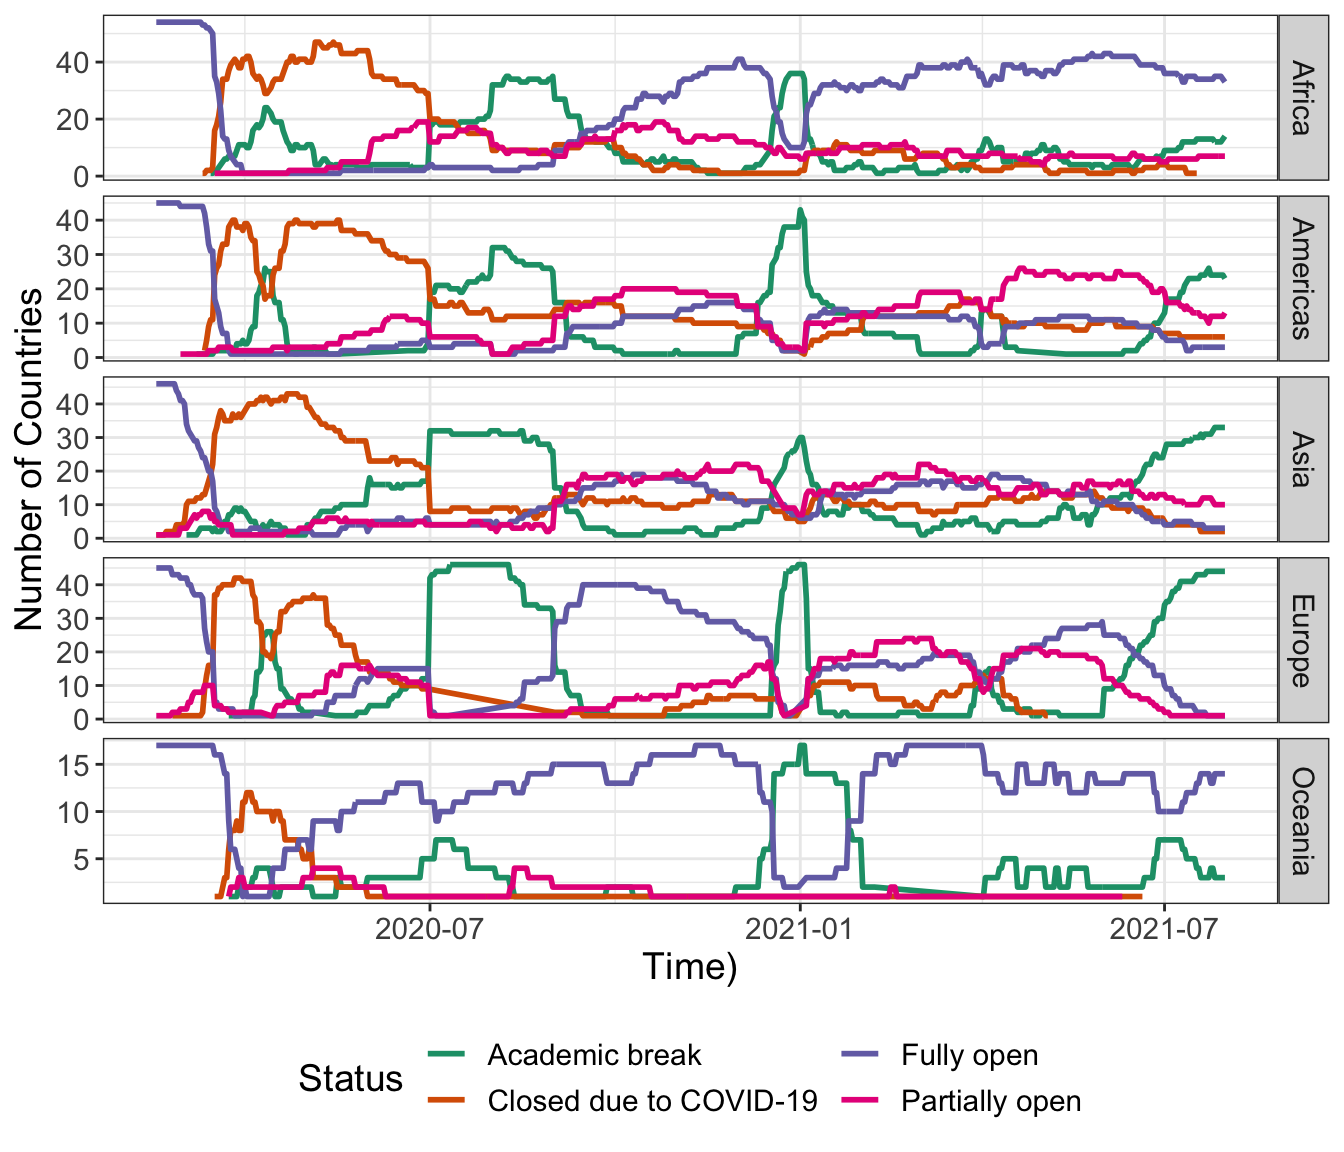
\includegraphics[width=1\textwidth]{figure/covidImpactContinent-1} 

}

\caption{Region wise tracking of COVID-19 caused school closures and re-openings}\label{fig:covidImpactContinent}
\end{figure}

The ongoing COVID-19 pandemic has brought the world to a standstill. Many sectors have been affected ever since the outbreak of COVID 19, worldwide. Among these many sectors education is one of the most affected sectors with a near-total closures of schools, colleges and universities, all around the world \autocite{daniel2020education}. Figures \ref{fig:covidImpactWorld} shows the evolution of global school closures and reopening since mid February 2020. With the start of the pandemic a near total closure of schools were observed all around the world. Over time, Africa and Oceania demonstrated better recovery in comparison to other regions with their increasing number of fully open schools (Figures \ref{fig:covidImpactContinent}).

\begin{figure}[h]

{\centering 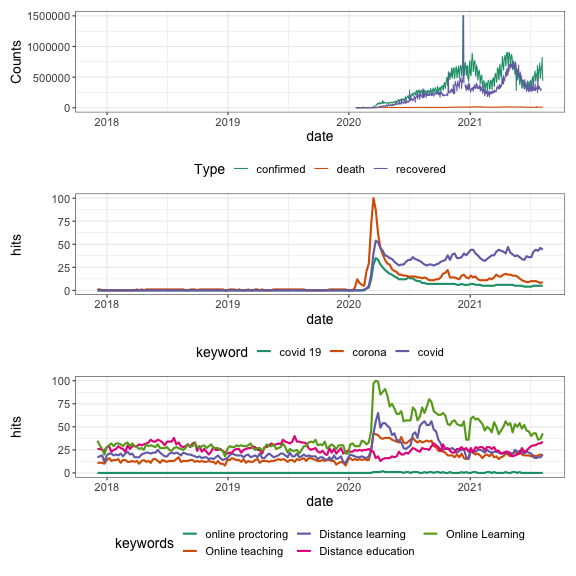
\includegraphics[width=1\textwidth]{figure/distanceLearningWorldAnalysis-1} 

}

\caption{Visualization of data from Goolge search trends. (a) COVID-19 cases worldwide (b) Google search trends of COVID-19 related terms (c) Google search trends of distance education related terms.}\label{fig:distanceLearningWorldAnalysis}
\end{figure}

Eventhough distance education has a long history that goes back to almost two centuries with significant modifications,
alterations, and addition in the process of delivery and communication \autocite{moore2011learning,spector2014handbook}, COVID 19 certainly made a new era of distance education while encouraging various stakeholders of education to take the concept of distance education seriously. Sudden unexpected movement from classrooms to home schooling at large scale made students, teachers and parents vulnerable, leading to millions of education related internet searches being performed during the period of COVID 19 pandemic (Figures \ref{fig:distanceLearningWorldAnalysis}). Surprisingly, the search spikes of distance education related searches (Figure \ref{fig:distanceLearningWorldAnalysis} (c)) coincide with increasing Covid-19 counts (Figure \ref{fig:distanceLearningWorldAnalysis} (a)) and related internet searches (Figure \ref{fig:distanceLearningWorldAnalysis} (b)), eventhough distance education has a long history in contrast to Covid-19 pandemic.

The speed of the physical classroom closures and the rapid move to online delivery of education allowed little time for planning or reflection on potential risks that could happen to its various stakeholders: teachers, students and parents. Teachers were not fully aware of their obligations and how to maintain connections with students to support thier learning. Lack of preparation, lack of tools and techniques for distance education, lack of awareness of the availability of the existing tools and techniques and their effectiveness, lack of interaction and communication with the students, lack of awareness of students' ongoing problems were some of the major issues they encountered during COVID 19 pandemic. Students on the other hand who tend to have fewer educational opportunities beyond schools and universities severely affected from this sudden unexpected movement. Further, the impact was not limited to students' learning but also to other aspects of their lives such as student debt, digital exclusion, lack of technology, lack of access to internet-enabled device or a stable internet connection, long-term educational disengagement, poor nutrition and food insecurity, increased psychological challenges, childcare problems, exploitation, school dropouts and lack of disability services. \autocite{drane2020impact,daniel2020education,unescoadverse2020}. This also put an extra burden on parents, specially with limited education and resources, as they were expected to facilitate the required learning environment at home. Further, every single step including planning, developing new tools and techniques, conducting awareness programmes about distance education, shifting towards distance education, happened through online, due to the unexpected massive global shutdown. This situation left internet as the only medium to support all these educational processes.

In response to this gray situation and urgent requirement of massive transformation from physical classroom to virtual learning environment, UNESCO took immediate and timely action by publishing a long list of distance learning solutions that can be used to facilitate student distance learning during the period of school closure. There are many different distance learning solutions. The design of different types of distance learning solutions can depend on the learning objective, target audience, access, and type of content \autocite{moore2011learning}. However, getting familiar with all these available distance solutions is not feasible or practical due to limited time availability and need of urgent responses.

According to \textcite{ahn2006utilizing}, the popularity of a product greatly influences consumer purchasing decisions. It can also indicate the prominence of the product in the market, its usability and its impact. Further, according to \textcite{willis2020using}, developers also tend to improve their products and services in response to increasing online search. Therefore, the internet represents a great opportunity to learn about public attention towards a product or service. It is also a way to narrow down the search space and thereby identify most suitable product and services that meets customer needs.

Google Trends is an open source web analytics tool that allows users to interact with Internet search data, which can provide deep insights into population behavior \autocite{nuti2014use}. In this study we test whether the Google Analytics search index series can be used as a proxy of the popularity and the public interest in different distance education solutions. In line with that, this paper makes three fundamental contributions to distance education by exploring three main questions: (1) What is the impact of COVID 19 pandemic on education? (2) What solutions are in place to meet the need of distance education in terms during COVID 19 pandemic? (3) Which distance learning solutions have a wide attention and public interest during the COVID-19 pandemic?
We primarily analyze quantitative digital footprint data on the internet from December 2019 to August 2021. The resulted google trend footprint provides a fast first step to identify the most popular distance education tools available for different education purposes. It also allows the teachers to narrow down the search space and deepen their exploration on prominent distance education solutions to support their online teaching.

Quality education is essential to sustainable development and it is a key United Nations (UN) sustainable development goal. Having the right tool is imperative to successful completion of a task at hand. The findings of this study provides an initial guidance to select a right tool. Therefore, the findings of this study directly contribute to UN's sustainable development goals of quality education.

The remainder of this paper is organized as follows. Section 2 presents the related work to lay the foundation for the Google footprint analysis. Section 3 presents the methodology followed in the study. Section 4 includes Google footprint analysis. Section 5 concludes the article and presents future research directions.

\hypertarget{background}{%
\subsection{Background}\label{background}}

\hypertarget{analysis}{%
\subsection{Analysis}\label{analysis}}

\hypertarget{discussion-and-conclusion}{%
\subsection{Discussion and Conclusion}\label{discussion-and-conclusion}}

\printbibliography

\end{document}
